\chapter{Introducing software performance engineering}
\label{cpt:software_performance_engineering}

In this chapter we look into the topic of introducing software performance engineering (SPE) into Tribler by adding a performance regression test system into the Tribler development cycle.
By looking at the tools already available and prior work, we come up with a system that is both extensive and has minimal impact in Tribler's current architecture.
By comparing two version of Tribler, one with the asynchronous I/O rework done in this thesis and Tribler's current code base, we show that this performance regression test system is an asset to Tribler from which many future developers can benefit in the coming years.
Moreover, this performance regression test system should force developers to keep an eye on performance when making code changes, gradually improving Tribler performance over time.

\section{Introduction to Gumby}
\label{sct:gumby_introduction}
%\begin{figure}[h]
%	\makebox[\textwidth][c]{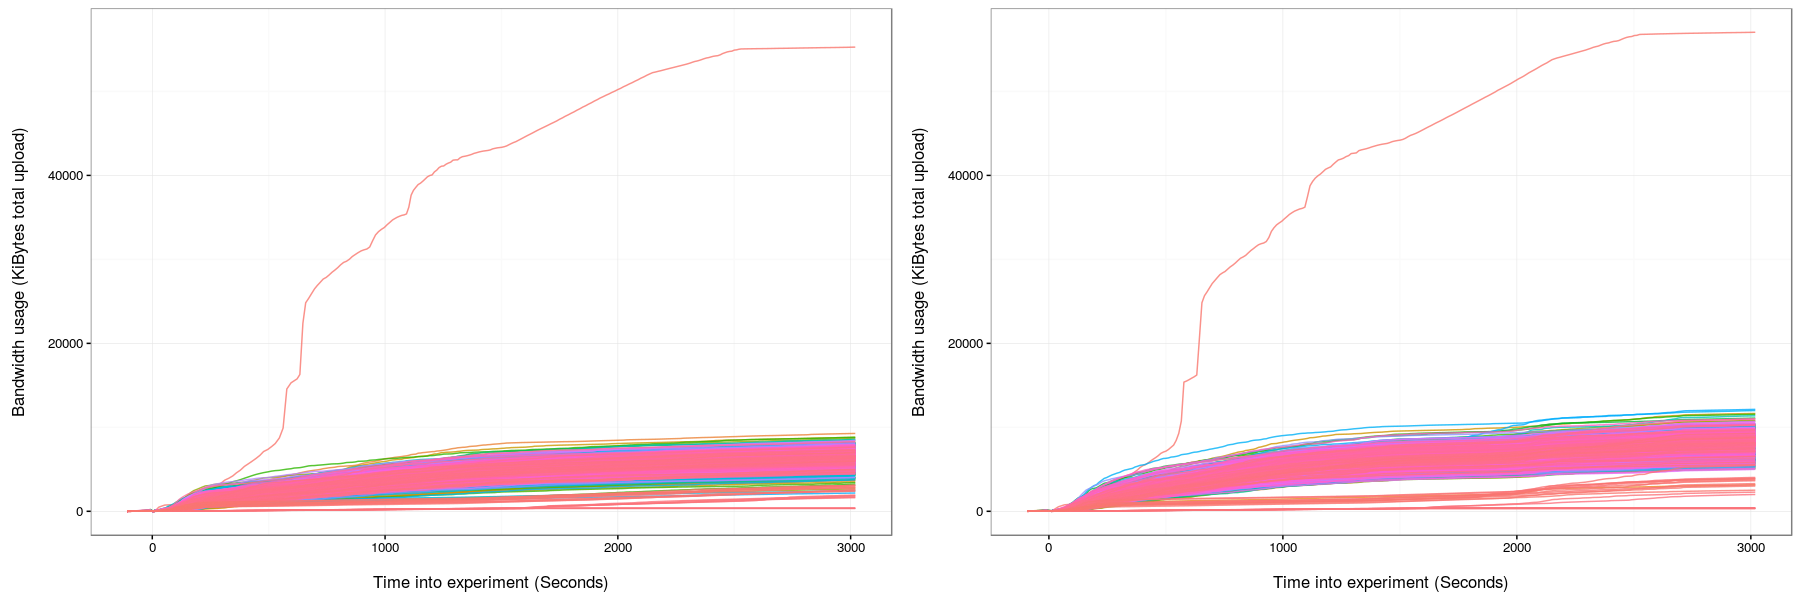
\includegraphics[width=\linewidth]{experimentation/images/send.png}}
%	\caption{An example of a side by side comparison of two \enquote{allchannel} experiment runs. Left the current code base, right asynchronous Dispersy with blocking I/O.}
%	\label{fig:side_by_side_send}
%\end{figure} 

Gumby is an experiment runner framework for Dispersy and Tribler.
It is being used by Tribler developers to run experiments on local computers as well as remote servers such as the DAS5 super computer\footnote{\url{http://www.cs.vu.nl/das5/}}.
Gumby takes care of most of the steps required in order to run an experiment, including:

\begin{itemize}
	\item Clearing the output directory at the start of an experiment.
	\item Syncing workspace directories with remote nodes.
	\item Run setup scripts concurrently to set up the experiment on all nodes.
	\item Spawn trackers to monitor the experiment and abort in case errors occur.
	\item Start both local and remote process instances in parallel at the exact same time.
	\item Fetch all the data from the output directories residing on remote servers.
	\item Run post-experiment scripts to generate items such as graphs and tables.
\end{itemize}

To run an experiment one can specify configurations and scenario files to be executed.

Configuration files specify which experiment to run and define all the settings needed in order to run this experiment using Gumby.
These settings often include paths to data, variables such as how many nodes to create and how long the experiment has to run.
Once a configuration file has been created, it can be passed to Gumby which takes care of running the experiment specified.

Scenario files allow for a carefully timed execution of functions.
In a scenario file, each line specifies which nodes executes which function at what time.
This is extremely useful in order to repeat the exact same procedure many times.

The combination of configuration and scenario files enable a setting in which a developer can run an experiment many times with the exact same execution order and timing.
This enables us to perform regression tests using Gumby which we will elaborate on next.

Whenever a push happens on a pull request on GitHub, our Jenkins continuous integration system can automatically schedule this experiment to be run. \todo{komt uit de lucht vallen}

Moreover, statistics such as CPU, memory consumption and I/O are automatically tracked by Gumby.
Any additional information that one wishes to track can be logged and parsed using auxiliary post experiment scripts.
All graphs are being generated in the R programming language using the ggplot2 library.

To realize a regression testing system, we decided to extend Gumby with additional functionalities and scripts.
First the proposed commits first have to be run inside a benchmark using a predetermined scenario and configuration file.
This will produce data about the changes made to the codebase.
Once this experiment is done, we can compare this data with the data generated by running the current code base using the same benchmark.
To create a comparison that requires little effort to interpret, graphs and tables will be generated and presented to the developer.
By creating a side-by-side plot of two graphs using the same scales, developers can immediately see any big changes, for a more in-depth view the developer can refer to the table which presents the results in a more fine grained fashion.

\section{Performance regression using Gumby}

By using configuration files and scenario files, we can create experiments which run Tribler and perform certain actions such as downloading content.
These experiments can in turn be used to compare different versions of Tribler which allows us to test for performance regression. 
To allow for such comparisons, we decided to extend Gumby by adding experiments or \emph{benchmarks} and additional data processing mechanisms.
This procedure works as follows.

First, we run the current version of Tribler or Dispersy i.e. the current code base using a certain benchmark which may spawn several nodes running this version.
Next, we run the exact same benchmark using the exact same amount of nodes on a modified version of Tribler or Dispersy.
Gumby will ensure that all functions will be called at the exact same moments, ensuring the execution of both runs is identical.
While the experiment is running, Gumby tracks statistics such as memory usage or response times and writes these to a specified output directory.
At the end of each experiment, all (relevant) data is fetched from the nodes and combined into a dataset.
Using post-experiments scripts we can then compare the data from the two obtained datasets and check if there are changes in e.g. resource usage or response times.

\section{Representative benchmarks}

One of the challenges of regression testing using benchmarks is that there should be benchmarks present which feature representative, real-world usage scenarios \cite{ferre2001usability}.
While it is intriguing to put a system to the limit of its capabilities and review if it performs better with made modifications, eventually real users should also profit from said modifications, improving the user experience of the software.
To provide developers with adequate scenarios, we have devised three benchmarks which feature a realistic use-case of Tribler.

\subsection{Benchmark 1}

The first benchmark that we have devised consists of a user having just installed the Tribler client and is about to join the network.
This use case is especially important for user satisfaction as first impressions add to this impression \cite{ferre2001usability}.

\begin{figure}[!h]
	\centering
	\includegraphics[width=0.6\linewidth]{regressiontesting/diagrams/bootstrap_procedure}
	\caption{The bootstrap procedure of Tribler.}
	\label{fig:tribler_bootstrapping}
\end{figure}

When a new client joins the network it has no knowledge of this network yet besides the location of bootstrap servers which are hard-coded in the Tribler client.
To gather information about the network and to start discovering peers and content, the client connects to the bootstrap servers, requesting the locations of peers in the network to exchange data with.
After the bootstrap client provides this information, the client will connect to these peers and start exchanging information about content and peers.
This process is visualized in Figure~\ref{fig:tribler_bootstrapping}.
Over time, this new peer will learn of all content in the network.

By running a Tribler client with no prior knowledge idle for a fixed amount of time, measurements on Tribler's resource usage such as CPU and I/O rates can be tracked.
As Dispersy facilitates Tribler's peer and content discovery, all data will be written to a SQLite database which generates I/O.
Meanwhile incoming messages are processed which creates CPU load.

To create this benchmark, an old experiment that runs Tribler idle has been fixed.
This experiment was introduced by a Tribler developer to run Tribler for various amounts of time, ranging from 1 hour to 1 week, at set times.
Unfortunately it was not updated when changes were made to Tribler.
By updating this experiment, it is now functional again and can be run using the latest version of Tribler and Dispersy.

\subsection{Benchmark 2}

The second benchmark represents a user downloading content by opening a magnet link or torrent file using Tribler, closing it as soon as it's finished downloading.
This benchmarks represents the free-riding problem: users downloading content without uploading it back to the network i.e. seeding \cite{adar2000free}.
To mimic this behaviour, we start Tribler and immediately start downloading a file using a magnet link, as if someone opened a magnet link from a third party website.
By periodically checking the download status, Tribler can be shutdown when the download is complete.

Using this benchmark, statistics such as CPU usage and download rates can be measured between different versions.
This provides insight into Tribler's core functionality: decentralized access to distributed content.

To implement this, the code of the first benchmark was used as a foundation, adding the download, download progress check and shutdown procedure logic to it.

\subsection{Benchmark 3}
\label{ssct:benchmark_3}

In this third benchmark we stress test Tribler by performing requests to the newly introduced application programming interface (API).
This API is work that is being done in parallel to this thesis by other members of the Tribler development team where the graphical user interface (GUI) is decoupled from Tribler's core logic.
This GUI will instead run in a separate process, communicating through a socket with Tribler's core, allowing Tribler to run headless i.e. without a GUI.

Somewhat related to the first benchmark, the response times of this API are equally important.
Hassenzahl et al. show that web designers have 50 milliseconds to make a good first impression \cite{lindgaard2006attention}.
Just like most websites, Tribler's user interface will receive data from an API, rendering response times of this API an important factor.
Especially when the GUI has just been opened on a fresh install, various requests will be send to API requesting channels, torrents, upload and download rates, the amount of free space on the machine, etc.
Meanwhile Tribler's core will also be busy connecting to the bootstrap servers as previously discussed.
To still deliver good response times, Tribler's core should be as responsive as possible to process incoming requests to this API as fast as possible.

To measure the responsiveness of this API, and indirectly that of Tribler, we have created a benchmark which can perform a varying amount of requests per second to Tribler's API.
To perform these requests, we have used Apache JMeter\footnote{\url{http://jmeter.apache.org/}}.
Apache JMeter was designed to "simulate a heavy load on a server, group of servers, network or object to test its strength or to analyse overall performance under different load types." (jmeter.apache.org, 2016).
JMeter tracks the average, maximal en minimal response times and calculates the standard deviation.
Additionally, it tracks how many responses are received per second and what the throughput of the API is.

By running this benchmark on two different versions of Tribler, we can observe if the are changes in any of the mentioned statistics captured by JMeter.
Since the responsiveness is directly related to the performance of a program, this will provide a good indication.


\section{Continuous regression testing using Jenkins}

To include software performance engineering in Tribler's development cycle, it was decided to include regression testing in our Jenkins continuous integration system.
Using Jenkins, one can create jobs to run specific tasks.
Examples of this is checking out the current version of Tribler using git and running the unit tests on this version.
Additionally, Jenkins can automatically run jobs on defined events such as commits pushed to a pull request or a new pull request being opened on the GitHub repository.

At the start of this thesis, Jenkins would only run unit tests on a Linux server.
To be able to run tests on all major platforms Tribler supports, three additional servers were set up running Windows 32-bit, Windows 64-bit and OS X Yosemite, respectively.
After these were deployed a code coverage and pylint checker job were added which track how much of the code has been tested and if the code adheres the PEP8\footnote{\url{https://www.python.org/dev/peps/pep-0008/}} code style, respectively.
When either the code coverage drops or the pylint check fails, the build is marked as failed, safeguarding deterioration of the code base.

To further improve Tribler's development process, we have created a performance regression job that runs the third benchmark using five requests per second.
To merge this job into the development cycle, we have prepared it to be added to the \enquote{GH\_Tribler\_PR} MultiJob.
This \enquote{GH\_Tribler\_PR} MultiJob runs whenever a user pushes a commit to an open pull request, forces a rerun or opens a new pull request on GitHub.
Whenever this performance regression job fails, indicating performance regression has occurred, the \enquote{GH\_Tribler\_PR} is marked as failed.
Upon failure, the author who proposes the changes must then investigate and adjust the code accordingly.

To be able to compare old and new code, we have created a separate job that runs the current code base of Tribler daily using the same experiment.
Using this job, we can command Jenkins to fetch the data from this job so we can create a comparison graph and table depicting changes between the outputs of each job.
Once this job is added to the MultiJob, whenever a pull requests gets merged into the code base, this job will automatically run again to ensure comparisons happen against the most recent version.

To make sure the build server can process all jobs in parallel without running out of resources, each server has a specific amount of slots defined.
In Jenkins, every job that is running takes up a slot on a build server.
To avoid allocating too many slots at once, the \enquote{GH\_Tribler\_PR} MultiJob consists of three phases:

\begin{enumerate}
	\item The first phase is the testing phase. In this phase tests are run on the four build servers and in parallel the code style is being checked. Because the current code base is under heavy maintenance by other members of the Tribler team, the next phase is always entered to obtain coverage information.
	\item The second phase is the code coverage phase. After the tests have run, all code coverage statistics are merged together to obtain the full coverage report. Next, the full report is compared against the full report of the current code base. If the code coverage dropped with this version, the build is marked as failed, otherwise the third and final phase is entered.
	\item The third phase is the experimental phase. In this phase an experiment called \enquote{Allchannel+ChannelCommunity\_short} is run which checks if Dispersy can still synchronize data properly.
\end{enumerate}

\begin{figure}[!h]
	\centering
	\includegraphics[width=\linewidth]{regressiontesting/diagrams/three_stages_testing}
	\caption{The three stages of testing}
	\label{fig:three_stages_of_testing}
\end{figure} 

As our benchmark can be categorized as experiment, we decided to add our job to the third phase.
Figure~\ref{fig:three_stages_of_testing} visualizes the three phases of the \enquote{GH\_Tribler\_PR} MultiJob.

\subsection{Multiple platforms}

\begin{figure}[!h]
	\centering
	\includegraphics[width=0.6\linewidth]{regressiontesting/diagrams/jenkins_multiple_os}
	\caption{Jenkins running on four major operating systems.}
	\label{fig:jenkins_multiple_os}
\end{figure} 

As each of these operating systems could influence performance \cite{gupta1991impact}, it is evident regression testing should be performed on these operating systems.
Currently, the build servers are used to package Tribler for official releases and to run unit tests on.
Soon a build server running the Android operating system will be added as there is an official Android Tribler app in development.

Using Jenkins, we can schedule benchmarks automatically on all available servers, visualized in Figure~\ref{fig:jenkins_multiple_os}.
By doing so, we can observe if Tribler performs the same on all operating systems.
In case a specific operation system does not match the signature of the others, developers can look into the inner workers of this operating system to better understand the situation.
As this item was not feasible to implement giving the time left of this thesis, it is noted down as future work.